% Created 2023-06-21 mer. 16:41
% Intended LaTeX compiler: pdflatex

% =================================BASE====================================%
\documentclass[10pt]{article}
\usepackage[left=2cm,right=2cm,top=2cm,bottom=2cm]{geometry} % Marges
%\usepackage{libertine}
%\usepackage{libertinust1math}
\usepackage[T1]{fontenc} % Nécessaire avec FrenchBabel
\usepackage[utf8]{inputenc} % Important pour symboles Francophones, é,à,etc

\usepackage{lmodern}
\renewcommand{\familydefault}{cmr} % La meilleure police (CMU Serif Roman) (Je me suis battu).

\usepackage{natbib} % Bibliographie
\bibliographystyle{abbrvnat}



\usepackage{amsmath, amssymb, amsthm} % Symb. math. (Mathmode+Textmode) + Beaux théorèmes.

\usepackage{mathtools,cancel} % Utilisation de boîtes \boxed{} + \cancelto{}{}
\usepackage{graphicx, wrapfig} % Géstion des figures.
\usepackage{hyperref} % Permettre l'utilisation d'hyperliens.
\usepackage{color} % Permettre l'utilisation des couleurs.
\usepackage[dvipsnames]{xcolor} % Couleurs avancées.
\usepackage{titling} % Donne accès à \theauthor, \thetitle, \thedate

% >>> Physique >>>
\usepackage{physics} % Meilleur package pour physicien. 
\usepackage{pxfonts} % Rajoute PLEIN de symboles mathématiques, dont les intégrales doubles et triples
% <<< Physique <<<

\usepackage{lipsum} % For fun
\usepackage{tikz} % Realisation de figures TIKZ.
\usepackage{empheq} % Boite autour de MULTIPLE équations

\usepackage[french]{babel} % Environnements en Français.
% ==============================BASE-(END)=================================%



% ================================SETTINGS=================================%
% Pas d'indentation en début de paragraphe :
\setlength\parindent{0pt} 

% Couleurs de hyperliens :
\definecolor{mypink}{RGB}{147, 0, 255}
\hypersetup{colorlinks, urlcolor=mypink, citecolor=mypink, linkcolor=mypink}

% Numéros d'équations suivent les sections :
\numberwithin{equation}{section} 

% Les « captions » sont en italique et largeur limitée
\usepackage[textfont = it]{caption} 
\captionsetup[wrapfigure]{margin=0.5cm}


% Retirer le l'écriture en gras dans la table des matières
\usepackage{tocloft}
\renewcommand{\cftsecfont}{\normalfont}
\renewcommand{\cftsecpagefont}{\normalfont}

% Change bullet style
\usepackage{pifont}
\usepackage{enumitem}
\setlist[itemize,1]{label=\ding{224}}
% ================================SETTINGS=================================%



% ==============================NEWCOMMANDS================================%
% Degrés Celsius :
\newcommand{\celsius}{${}^\circ$ C} % \degrée Celsius : Pas mal plus simple qu'utilise le package gensymb qui plante avec tout...

% Vecteurs de base :
\newcommand{\nvf}{\vb{\hat{n}}}
\newcommand{\ivf}{\vb{\hat{i}}}
\newcommand{\jvf}{\vb{\hat{j}}}
\newcommand{\kvf}{\vb{\hat{k}}}

\newcommand{\uu}{\vb*{u}}
\newcommand{\vv}{\vb*{v}}

% Boîte vide pour ajuster les underbrace
\newcommand{\bigno}{\vphantom{\qty(\frac{d}{q})}}
\newcommand{\pt}{\hspace{1pt}}

% Physics empty spaces 
\newcommand{\typical}{\vphantom{A}}
\newcommand{\tall}{\vphantom{A^{x^x}_p}}
\newcommand{\grande}{\vphantom{\frac{1}{xx}}}
\newcommand{\venti}{\vphantom{\sum_x^x}}

% Moyenne numérique entre deux points de grilles. 
\newcommand{\xmean}[1]{\overline{#1}^x}
\newcommand{\ymean}[1]{\overline{#1}^y}
\newcommand{\zmean}[1]{\overline{#1}^z}
\newcommand{\xymean}[1]{\overline{#1}^{xy}}

% Tilde over psi
\newcommand{\tpsi}{\tilde{\psi}}

% Nota Bene env :
\newcommand{\nb}{\textbf{N.B.}\hspace{4pt}}
   
% ==============================NEWCOMMANDS================================%



% ==============================PAGE-TITRE=================================%
% Titlepage 
\newcommand{\mytitlepage}{
\begin{titlepage}
\begin{center}
{\Large Contrat Été 2023 \par}
\vspace{2cm}
{\Large \MakeUppercase{\thetitle} \par}
\vspace{2cm}
RÉALISÉ DANS LE CADRE\\ D'UN PROJET POUR \par
\vspace{2cm}
{\Large ISMER--UQAR \par}
\vspace{2cm}
{\thedate}
\end{center}
\vfill
Rédaction \\
{\theauthor}\\
\url{charles-edouard.lizotte@uqar.ca}\\
ISMER-UQAR
\end{titlepage}
}
% ==============================PAGE-TITRE=================================%



% =================================ENTÊTE==================================%
\usepackage{fancyhdr}
\pagestyle{fancy}
\setlength{\headheight}{13pt}
\renewcommand{\headrulewidth}{1.3pt} % Ligne horizontale en haut

\fancyhead[R]{\textit{\thetitle}}
\fancyhead[L]{\ \thepage}
\fancyfoot[R]{\textit{\theauthor}}
\fancyfoot[L]{}
\fancyfoot[C]{} 
% =================================ENTÊTE==================================%
\author{Charles-Édouard Lizotte}
\date{23/06/2023}
\title{Carnet de bord, Université McGill}
\hypersetup{
 pdfauthor={Charles-Édouard Lizotte},
 pdftitle={Carnet de bord, Université McGill},
 pdfkeywords={},
 pdfsubject={},
 pdfcreator={Emacs 28.2 (Org mode 9.6.5)}, 
 pdflang={French}}
\begin{document}

\mytitlepage
\tableofcontents\newpage



\section{{\bfseries\sffamily TODO} Diagnostiques utiles}
\label{sec:orgb5e89cc}

Concrétement, on se souvient que les diagrammes de Hovmoller pour le modèle \emph{shallow water} résolu à l'aide du \emph{package} MUDPACK sont illustrés dans le \href{rapport-2023-06-16.org}{dernier rapport}.
Pour en avoir un avant goût, la figure \ref{fig:org763f1d1} illustre l'état de la situation.
Essentiellement, tout se passe bien, mais des lignes horizontales viennent remettre en doute nos résultats.
Le \emph{spin up} du modèle arrive au bon moment (aux alentours de 800 jours, comme on l'observe dans le modèle résolu par transformées de Fourrier).
Ces lignes verticales sont particulièrement visible dans le rotationnel du courant. 

\begin{figure}[htbp]
\centering
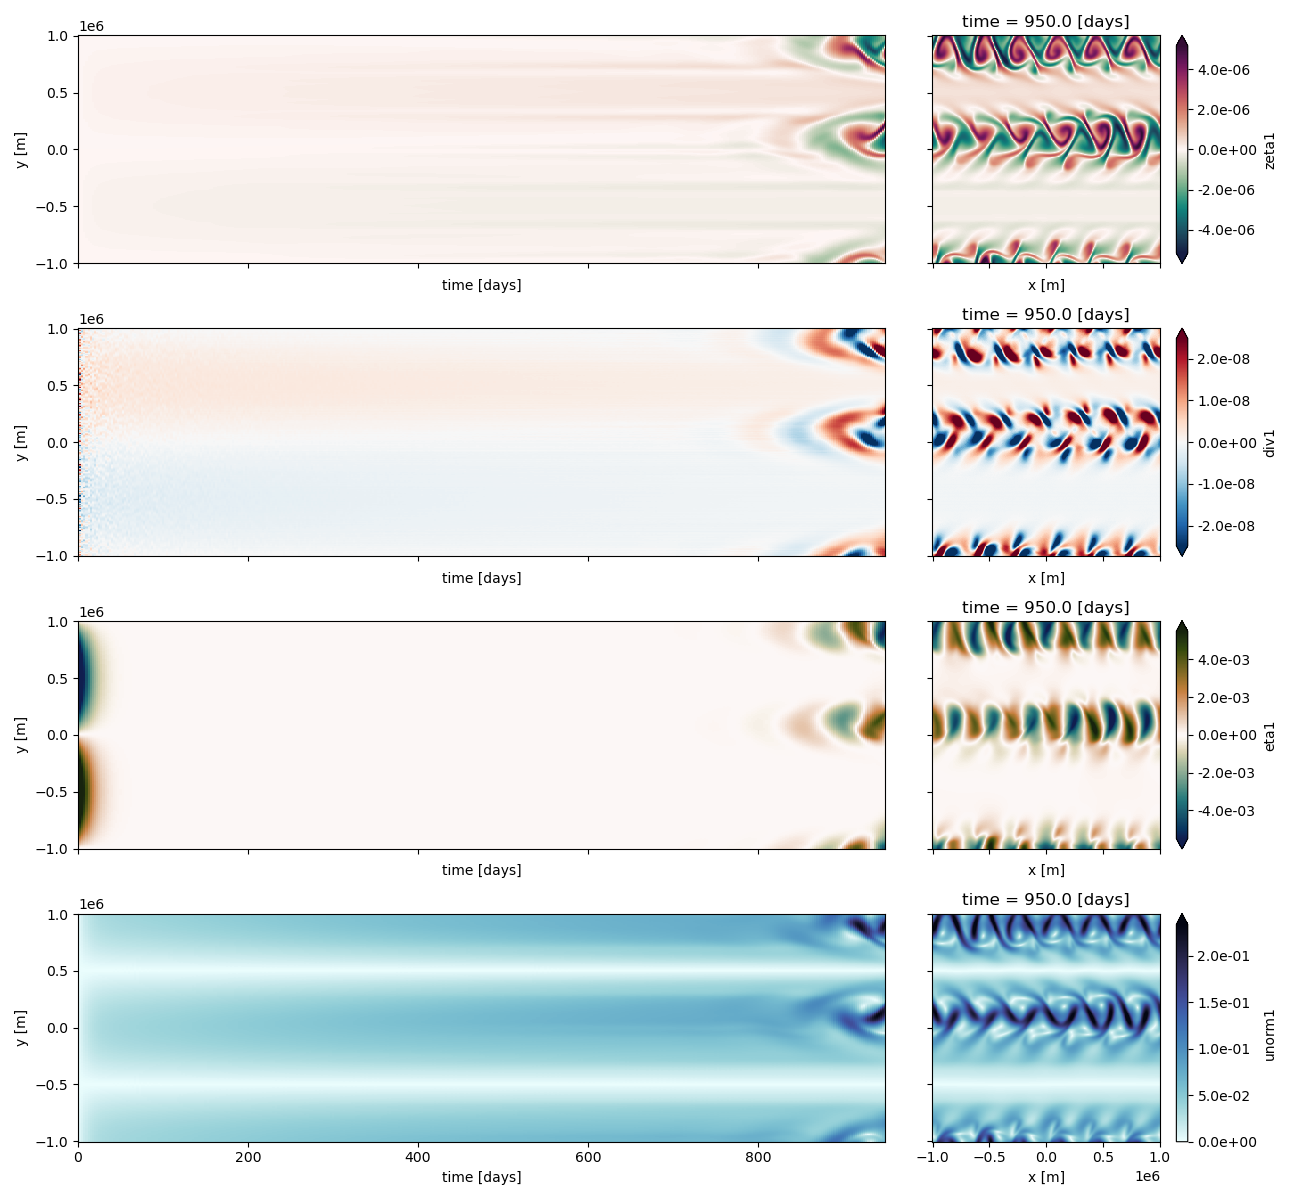
\includegraphics[width=.9\linewidth]{figures/tests/2023-06-21_hovmoller1_t=950days.png}
\caption{\label{fig:org763f1d1}Diagrame de Hovmoller entre 0 et 950 jours pour le modèle shallow water résolu par MUDPACK. Du haut vers le bas, la vorticité, la divergence, la correction à la fonction de courant barotrope et la norme du courant. Le tout pour la première couche.}
\end{figure}



\subsection{{\bfseries\sffamily DONE} Divergence du transport barotrope}
\label{sec:orgda1c814}
Notre première hypothèse : La solution obtenue avec MUDPACK ne se trouve pas en résolvant l'équation de la conservations de la masse, qui donnée par
\begin{equation}
\label{eq:org993bfc1}
   \div{\uu_{BT}} = 0,
\end{equation}
mais plutôt en solvant l'équation de fonction de courant géostrophique, donnée par
\begin{equation}
   \laplacian{\psi_{BT}} = \kvf \cdot \zeta_{BT}.
\end{equation}
Donc il faudrait vérifier que l'équation \ref{eq:org993bfc1} (la conservation de la masse) est bel et bien respectée.\bigskip

Pour se faire, j'ai du relancer quelques \emph{runs} car ne sortais que les \emph{output} de la première couche pour sauver de l'espace sur mon ordinateur.
Les résultats sont là :
La divergence du transport barotrope est \emph{plutôt très} nulle, ce qui veut dire que la conservation de la masse (\ref{eq:org993bfc1}) est respectée.

\begin{figure}[htbp]
\centering
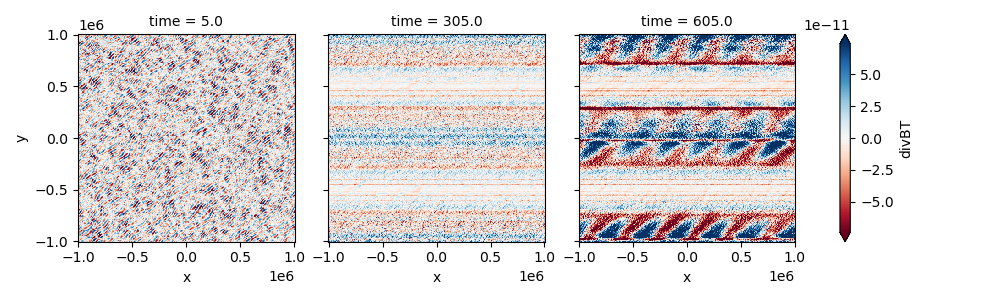
\includegraphics[width=.9\linewidth]{figures/debuggage/2023_06_21divBT1.png}
\caption{\label{fig:orgaf83ab7}Divergence du courant barotrope à divers moments.}
\end{figure}
\begin{figure}[htbp]
\centering
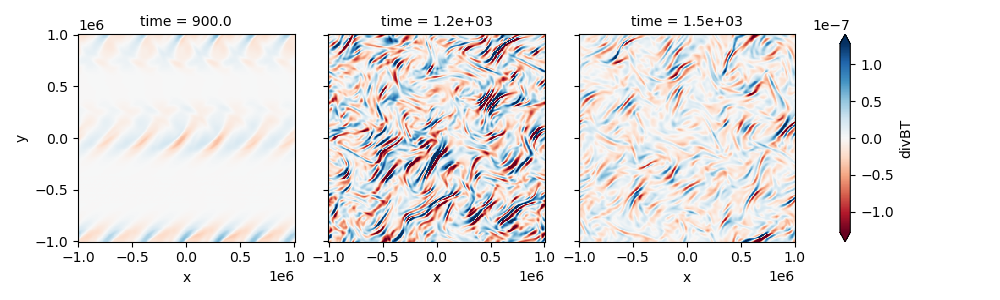
\includegraphics[width=.9\linewidth]{figures/debuggage/2023_06_21divBT2.png}
\caption{\label{fig:orgaf83ab7}Divergence du courant barotrope à divers moments.}
\end{figure}



\subsection{{\bfseries\sffamily TODO} Effet du filtre de Robert}
\label{sec:org059108e}
\subsection{{\bfseries\sffamily TODO} Contrainte de cisaillement du vent moins forte}
\label{sec:org0d8778d}


\section{{\bfseries\sffamily TODO} Problème conceptuel avec MUDPACK?}
\label{sec:orga02ca3e}
\subsection{Les tests de MUDPACK}
\label{sec:org52c3c33}
\subsection{Est-ce que MUDPACK prend un point à la fin? Que dit la documentation?}
\label{sec:orgbb2cb48}
\end{document}